\subsection{Base de Dados}

Primeiramente, a base de dados oferecida consistia em $10$ arquivos \textit{.jpg} de teste e $10$ arquivos \textit{.jpg} de treino, o i-ésimo arquivo se refere a um grande conjunto de imagens do digito $i$, portanto dentro do arquivo \textit{mnist\_train\_0} tem vários digitos $0$, cada digito $0$ está contido em um quadrado de $28$ por $28$ pixels, discretizado pela intensidade de sua cor entre $0$ e $255$. Cada imagem foi separada em um vetor coluna de dimensão $28\times28 = 784$.

\begin{figure}[!h]
    \centering
    
\includegraphics[scale=0.4]{Imagens/digito5.jpg}
    \caption{Exemplo do digito $5$ do conjunto MNIST}
    \label{fig:5}
\end{figure}

Em \textit{machine learning} é interessante que se normalize os dados para processamento, uma vez que os classificadores binários julgam valores de $0$ e $1$, portanto, os dados de imagem de $0$ a $255$ foram normalizados pelo fator de $255$.

\subsection{Hiperparâmetros}

A rede neural MLP foi elaborada de forma totalmente conectada vide Figura \ref{mlp} utilizando $2$ camadas, onde a primeira camada possui $15$ neurônios e a segunda possui $10$ neurônios, onde a primeira camada possui função de ativação ReLU, e a segunda camada, que é a de saída possui a função de ativação sigmoide, mostradas na Figura \ref{ativacao}. A justificativa para essas escolhas é que um dos objetivos é mostrar que uma rede neural simples pode ter um bom rendimento, e também a resolução da lista $2$ utilizou a mesma rede, porém a saída era diferente, apenas classificava se estava contido ou não em um conjunto, no presente projeto, criou-se um vetor de dimensão $10$, onde se o elemento $i$ é $1$ e o resto $0$, então o digito representado por essa saída é $i$, logo se adaptou a rede para ter $10$ neurônios na saída. 

\begin{figure}[!h]
    \centering
    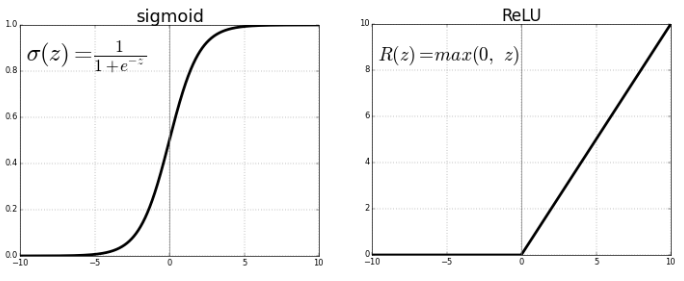
\includegraphics[scale=0.35]{Imagens/ativacao.png}
    \caption{Funções de ativação usadas}
    \label{ativacao}
\end{figure}


A taxa de aprendizagem usada no projeto foi $\alpha = 5\times 10^{-4}$ decidida pós análise da validação e de um teste de $5$ valores randomizados entre $10^{-4}$ e $10^{-6}$. Ademais, o modo de treinamento foi o Gradiente Descendente Estocástico, uma vez que buscava-se também que o treinamento fosse mais rápido, e o número de épocas, decidido também ao randomizar 5 valores entre $1$ e $10$, a quantidade de épocas que melhor se adequou ao projeto foi $10$.

\begin{figure}[!h]
    \centering
    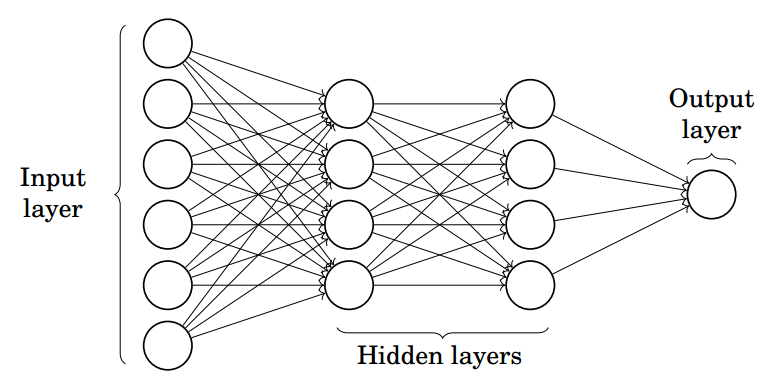
\includegraphics[scale=0.40]{Imagens/neural.png}
    \caption{Arquitetura de uma MLP completamente conectada}
    \label{mlp}
\end{figure}
